\documentclass{article}
\usepackage{graphicx} % Required for inserting images
\usepackage{biblatex}
\addbibresource{citations.bib}
\usepackage{amsmath}
\usepackage{amssymb}
\usepackage{multirow}
% \usepackage{array}
\usepackage{caption}
\usepackage{subcaption}

\DeclareMathOperator{\erm}{ERM}
\DeclareMathOperator{\dro}{DRO}
\DeclareMathOperator*{\argmax}{arg\,max}
\DeclareMathOperator*{\argmin}{arg\,min}

\title{Robustness to Spurious Correlations via Distributionally Robust Neural Network}
\author{Rong Jiang$^*$, Chenfeng Li$^*$, Charles Mayville$^*$}
\date{May 2023}

\begin{document}

\maketitle
\def\thefootnote{*}\footnotetext{Alphabetical order.}\def\thefootnote{\arabic{footnote}}

\section{Introduction}
In classical machine leraning, models are typically trained to minimize the average loss of a training dataset, and then evaluated on a test dataset that is often assumed to be from the same distribution as the training one. In practice, such methodology is problematic due to two reasons: 1) the training distribution and the test distribution can be different; 2) methods that optimize over average performance may suffer low performance on rare and atypical instances. For example, it is observed that models can experience significant downgrading performance when distribution shift between training and test data occurs \cite{ds}. Besides, models that achieve high average performance can still fail on atypical examples or rely on spurious correlations \cite{atypical}. These issues raise safety and fairness concerns for building trustworthy machine learning systems in areas such as medical diagnosis and autonomous vehicles.

To tackle these challenges, \cite{duchi} develops a distributionally robust
stochastic optimization (DRO) framework, which seeks to optimize the worst case performance over a family of potential test distributions. While the DRO framework considered in \cite{duchi} addresses the issues of distribution shift and worst-case performance, it is restricted to convex predictive models with limited capacity, and therefore cannot satisfy the needs of modern machine learing where deep neural networks play a central role.

DRO in the context of overparameterized neural networks is studied in \cite{groupdro} They consider group DRO, where they
train models to minimize the worst-case loss over groups in the training
data, so as to prevent the model from learning spurious correlations and suffering high loss on certain
groups of data. Under the overparameterized regime, they find that models trained through both group DRO and empirical risk minimization (ERM) can achieve nearly zero training loss and high average test accuracy, but the worst-group test accuracies are low. They suggest this behavior is because the average generalization gap is small while the worst group one is large. However, by applying regularization to group DRO models, they show the former can outperform regularized and unregularized ERM models in worst-group test accuracies while retaining high average test accuracies. Their findings indicate while overparameterization might allow for good average performance, regularization is still needed for good worst-case performance in neural networks.

In this report, we critically evaluate the method in \cite{groupdro} on a newly generated dataset that their work does not cover. We consider the colored MNIST dataset where we assign a binary label to the image according to the digit and color the image based on its label. We find that regularized DRO models can outperform regularized and unregularized ERM models in worst-group test accuracies while maitaining relatively high average
test accuracies, which corroborates the results in \cite{groupdro}. One limitation of \cite{groupdro} is that they assume the test groups are all seen during training. This assumption might not be realistic in practice so we add unseen groups to our test data to further examine the performance of group DRO. We observe that group DRO with regularization has worst-group and average test accuracies very close to the ones in test data with all-seen groups. This shows the ability of regularized group DRO to prevent models from learning spurious correlations.

The report is organized in the following way: section 2 formally introduces the settings of ERM and group DRO. Section 3 contains the experiment results of our colored MNIST data. Section 4 conludes and discusses future directions.

\section{Setup}
Let $x\in\mathcal{X}$ be the input feature and $y\in\mathcal{Y}$ be the label. Denote our hypothesis family as $\Theta$, and $l:\Theta\times(\mathcal{X}\times\mathcal{Y})\rightarrow\mathbb{R}_+$ is the loss function. We assume our training data is sampled from some distribution $P$. In standard machine learning, we use  empirical risk minimization (ERM) to find
\begin{equation}
    \hat{\theta}_{\erm}=\argmin_{\theta\in\Theta}\mathbb{E}_{(x,y)\sim\hat{P}}[l(\theta;(x,y))],
\end{equation}
where $\hat{P}$ is the empirical distribution of $P$.

Rather than minimizing the average loss, DRO  minimizes the worst-case expected loss over a set of distributions $\mathcal{Q}$:
\begin{equation}\label{dro}
    \min_{\theta\in\Theta}\{R(\theta)=\sup_{Q\in\mathcal{Q}}\mathbb{E}_{(x,y)\sim Q}[l(\theta;(x,y))]\}.
\end{equation}
Ideally, we want $\mathcal{Q}$ to contain the test distribution so that our model can perform well on it. One way to choose $\mathcal{Q}$ is to consider a divergence ball around the training distribution \cite{duchi}. 
% But in practice, finding the appropriate $\mathcal{Q}$ to avoid overly pessimistic models can be hard [...]

In this report, we consider the group DRO formulation as in \cite{groupdro}. Prior knowledge of spurious correlations is used to define groups over the training data and $\mathcal{Q}$ is then defined using these groups. Concretely, let $\mathcal{Q}=\{\sum_{g=1}^mq_gP_g:q\in\Delta_m\}$, where $\Delta_m$  is the $(m-1)$-dimensional probability simplex and $P_g$ is the distribution of group $g$. In other words, $\mathcal{Q}$ is a set of mixture distributions and each component of the mixture distribution represents a group. Since a linear program attains its optimum at the vertex, the worst-case risk in (\ref{dro}) is equivalent to the worst group risk
\begin{equation}
    R(\theta)=\sup_{g\in[m]}\mathbb{E}_{(x,y)\sim P_g}[l(\theta;(x,y))].
\end{equation}
Thus, we can learn a group DRO model
\begin{equation}\label{group-dro}
    \hat{\theta}_{\dro}=\argmin_{\theta\in\Theta}\{\hat{R}(\theta)=\sup_{g\in[m]}\mathbb{E}_{(x,y)\sim \hat{P}_g}[l(\theta;(x,y))]\}
\end{equation}
where $\hat{P}_g$ is the empirical distribution of $P_g$. Here, we assume the training data consists of $(x,y,g)$ triplets but $g$ is not assumed to be observed at test time. Group DRO prevents the model from learning spurious correlations by optimizing the performance of the worst group where the misleading heuristics might not hold. However, (\ref{group-dro}) does not imply good test worst-group performance due to the worst-group generalization gap $\delta=R(\theta)-\hat{R}(\theta)$. We will examine the effect of regularization on $\delta$ in the following section.

\section{Experiment}
\subsection{Data}
We start by describing how we construct our dataset from the MNIST database. For each image, we label it as one of $\mathcal{Y}=\{0,1\}$ based on the digit ($y = 0$ for digits 0-4 and $y = 1$ for digits 5-9) and color it as one of $\mathcal{A}=\{\text{red},\text{green}\}$, with 0 more frequently appearing on red images and 1 more frequently appearing on green images. We thereby form $m=|\mathcal{A}|\times|\mathcal{Y}|=4$ groups, one for each $(a,y)\in\mathcal{A}\times\mathcal{Y}$. It is expected that models which learn the correlation between label and color in the training data will perform badly on groups where the relation does not hold and consequently on the worst-group loss $R(\theta)$.

Specifically, we first label the image based on its digit as described above and then flip its label with a probability of 0.25. Then, we color a image as red if its label is 0 and green if its label is 1. We flip the color of each image with a probability of $0.2$. We uniformly split the data into training and test sets so that the portion of each group within training data and test data are roughly the same, with a training size of $20000$ and test size of $5000$\footnote{In training data, group (red,0) has size 8181, $|(\text{red},1)|=1938$, $|(\text{green}, 1)|=7843$, and $(\text{green},0)=2038$. In test data, group (red,0) has size 2070, $|(\text{red},1)|=511$, $|(\text{green}, 1)|=1939$, and $(\text{green},0)=480$.}. We want to point out that the label flipping procedure can be viewed as incoporating corruption into the data. So the optimal accuracy should be $1-0.25=0.75$ (recall we flip the label with a probability of 0.25) and an accuracy higher than that in the training process would indicate that the model relies on the spurious correlation or memorizes the data.

\subsection{ERM v.s. DRO without regularization}
We start by comparing the performance of ERM models and DRO models without regularization added.
\begin{description}
    \item[ERM.] The ERM models achieve $80.0\%$ average training accuracy and $80.3\%$ average test accuracy \footnote{The test accuracy is slightly higher here because the portion of worst groups in test data is slightly less than that of the training data.}. However, the worst-group training accuracy is only $0.2\%$ and the worst-group test accuracy is $0.3\%$\footnote{Unlike \cite{groupdro} where they obtain nearly perfect worst-group training accuracy using ResNet50 as the underlying learner which is able to memorize the data, in our case ERM performs badly even in the worst group of the training data because we use a moderately-sized convolutional neural network as our underlying learner due to computational constraint.}. Clearly, ERM models merely learn the spurious correlation between label and color and therefore fail on the groups where this relation do not hold. 
    \item[DRO.] The DRO models obtain $91.7\%$ average training accuracy and $72.8\%$ average test accuracy. The worst-group training accuracy is $89.8\%$ and the worst-group test accuracy is $44.4\%$ (Table \ref{table:nreg}, Figure \ref{dro_nr}). We find that though DRO without regularization can outperform ERM in terms of worst-group accuracies, the worst-group generalization gap between training and test data is still large.
\end{description}

\begin{table}[h!]
\centering
\begin{tabular}{ |p{1cm}|p{2cm}|p{2cm}|p{2cm}|p{2cm}|  }
\hline
& \multicolumn{2}{|c|}{Average Accuracy} & \multicolumn{2}{|c|}{Worst-Group Accuracy} \\
\hline
 & ERM & DRO & ERM & DRO \\
\hline
Train & $80.0\%$ & $91.7\%$ & $0.2\%$ & $89.8\%$ \\
\hline
Test & $80.3\%$ & $72.8\%$ & $0.3\%$ & $44.4\%$ \\
\hline
\end{tabular}
\caption{Comparison of ERM and DRO models without regularization.}
\label{table:nreg}
\end{table}

\begin{table}[h!]
\centering
\begin{tabular}{ |p{1cm}|p{2cm}|p{2cm}|p{2cm}|p{2cm}|  }
\hline
& \multicolumn{2}{|c|}{Average Accuracy} & \multicolumn{2}{|c|}{Worst-Group Accuracy} \\
\hline
 & ERM & DRO & ERM & DRO \\
\hline
Train & $80.2\%$ & $73.9\%$ & $0.0\%$ & $70.7\%$ \\
\hline
Test & $80.3\%$ & $71.3\%$ & $0.0\%$ & $67.5\%$ \\
\hline
\end{tabular}
\caption{Comparison of ERM and DRO models with regularization.}
\label{table:reg}
\end{table}

\subsection{ERM v.s. DRO with regularization}
Next, we regularize both models by using $l_2$ penalty and compare their performance.
\begin{description}
    \item[ERM.]The ERM models get $80.2\%$ average training accuracy and $80.3\%$
    average test accuracy. Still, the worst-group training accuracy is only $0.0\%$ and the worst-group test accuracy is $0.0\%$. We find that adding regularization does not improve the performance of ERM.
    \item[DRO.] Under regularization, DRO models reach $73.9\%$ average training accuracy and $71.3\%$ average test accuracy. Note that we flip $25\%$ of the labels in both training and test data so the optimal accuracy should be $75\%$ theoretically, and an accuracy higher than it suggests the model is memorizing the data. The worst-group training accuracy is $70.7\%$ and the worst-group test accuracy is $67.5\%$ (Table \ref{table:reg}, Figure \ref{dro_reg}). We can see that regularization significantly reduces the worst-group generalization gap while retaining the average test accuracy.
\end{description}

\begin{figure}
\begin{subfigure}{.5\textwidth}
  \centering
  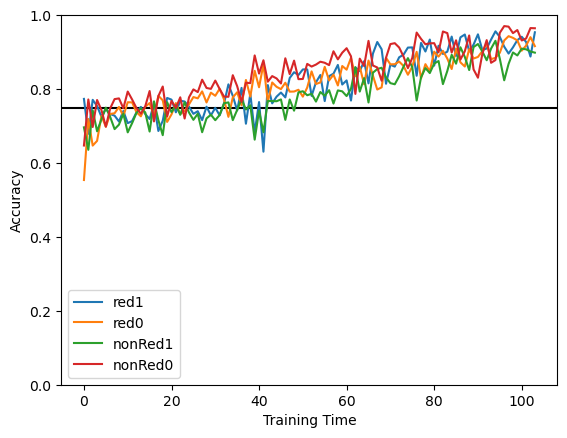
\includegraphics[width=1.\linewidth]{images/dro_train_nr.png}
  \caption{DRO training accuracy}
\end{subfigure}
\begin{subfigure}{.5\textwidth}
  \centering
  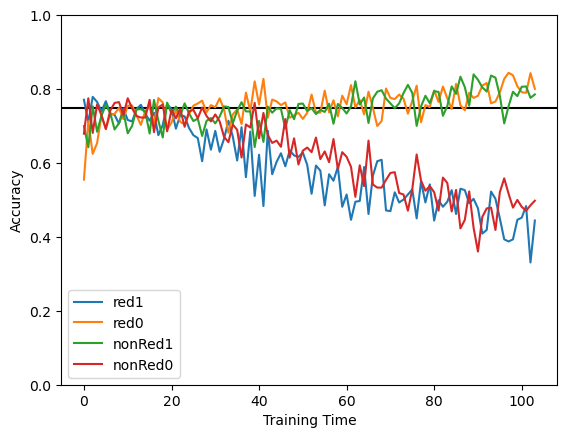
\includegraphics[width=1.\linewidth]{images/dro_test_nr.png}
  \caption{DRO test accuracy}
%   \label{fig:sfig2}
\end{subfigure}

\caption{Unregularized DRO accuracies by group (the black line at 0.75 represents the theoretical optimal accuracy)}
\label{dro_nr}
\end{figure}

\begin{figure}
\begin{subfigure}{.5\textwidth}
  \centering
  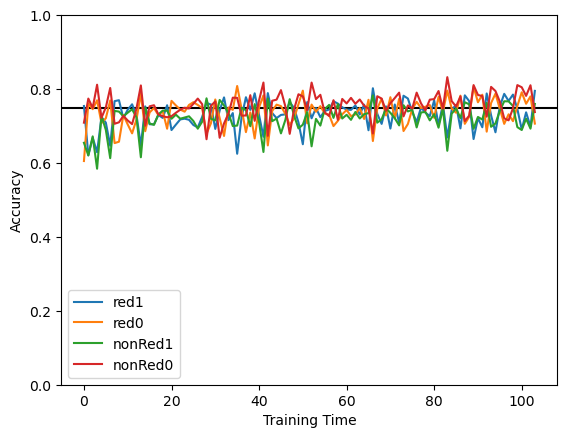
\includegraphics[width=1.\linewidth]{images/dro_train_reg.png}
  \caption{DRO training accuracy}
\end{subfigure}
\begin{subfigure}{.5\textwidth}
  \centering
  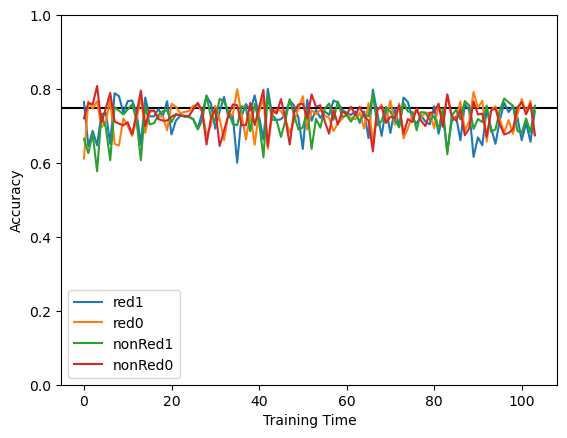
\includegraphics[width=1.\linewidth]{images/dro_test_reg.png}
  \caption{DRO test accuracy}
%   \label{fig:sfig2}
\end{subfigure}

\caption{Regularized DRO accuracies by group}
\label{dro_reg}
\end{figure}

\subsection{Unseen groups}
A limitation of \cite{groupdro} is that their test groups are all seen during training. To further evaluate DRO, we remove this condition and test it on unseen data. We do so by creating a test dataset with the originally green color replaced by random RGB values (Figure \ref{fig:unseen}). Using regularized DRO models trained on data containing only red and green groups, we obtain an average test accuracy of $69.8\%$ and a worst-group test accuracy of $67.3\%$ under the new test set with unseen groups. This result is similar to the result of regularized DRO on test data with all-seen groups. 

\begin{figure}[h]
\centering
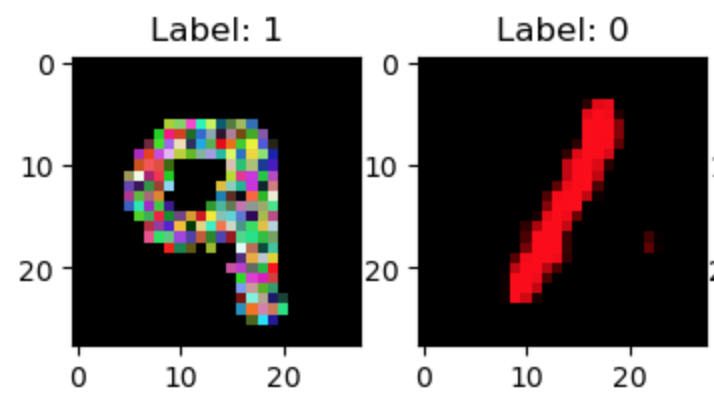
\includegraphics[scale=0.4]{images/unseen.png}
\caption{Unseen group where the green color is replaced by random RGB values}
\label{fig:unseen}
\end{figure}

\section{Discussion}
In this report, we examine the performance of group DRO on our colored MNIST dataset. We find that group DRO with regularization can improve the worst-group performance while keeping the average performance, which is consistent with the results in \cite{groupdro}. When evaluated on test data containing groups unseen during training, group DRO with regularization retains its worst-group and average test performance as before. This suggests group DRO with regularization has the potential to learn the underlying true relation instead of relying on spurious correlations. Nevertheless, group DRO has its limitations and more complicated real world data is required to fully test the effectiveness of it. For example, when we have multiple spurious feature values, we may need to split the data into many groups and could create tiny groups which might pose challenge to learning. Instead of focusing on the worst-group performance, methods which reweight different groups based on their training errors are also interesting solutions to the group distributional robustness problem \cite{liu2023ranking}. These directions are beyond the scope of this report and we leave them as future work.

\printbibliography

\section*{Appendix}
Our code is attached in the following pages.
\end{document}
